% Options for packages loaded elsewhere
\PassOptionsToPackage{unicode}{hyperref}
\PassOptionsToPackage{hyphens}{url}
\PassOptionsToPackage{dvipsnames,svgnames,x11names}{xcolor}
%
\documentclass[
  a4paper,
]{article}

\usepackage{amsmath,amssymb}
\usepackage{iftex}
\ifPDFTeX
  \usepackage[T1]{fontenc}
  \usepackage[utf8]{inputenc}
  \usepackage{textcomp} % provide euro and other symbols
\else % if luatex or xetex
  \usepackage{unicode-math}
  \defaultfontfeatures{Scale=MatchLowercase}
  \defaultfontfeatures[\rmfamily]{Ligatures=TeX,Scale=1}
\fi
\usepackage{lmodern}
\ifPDFTeX\else  
    % xetex/luatex font selection
\fi
% Use upquote if available, for straight quotes in verbatim environments
\IfFileExists{upquote.sty}{\usepackage{upquote}}{}
\IfFileExists{microtype.sty}{% use microtype if available
  \usepackage[]{microtype}
  \UseMicrotypeSet[protrusion]{basicmath} % disable protrusion for tt fonts
}{}
\makeatletter
\@ifundefined{KOMAClassName}{% if non-KOMA class
  \IfFileExists{parskip.sty}{%
    \usepackage{parskip}
  }{% else
    \setlength{\parindent}{0pt}
    \setlength{\parskip}{6pt plus 2pt minus 1pt}}
}{% if KOMA class
  \KOMAoptions{parskip=half}}
\makeatother
\usepackage{xcolor}
\usepackage[top=2.54cm,right=2.54cm,bottom=2.54cm,left=2.54cm]{geometry}
\setlength{\emergencystretch}{3em} % prevent overfull lines
\setcounter{secnumdepth}{-\maxdimen} % remove section numbering
% Make \paragraph and \subparagraph free-standing
\ifx\paragraph\undefined\else
  \let\oldparagraph\paragraph
  \renewcommand{\paragraph}[1]{\oldparagraph{#1}\mbox{}}
\fi
\ifx\subparagraph\undefined\else
  \let\oldsubparagraph\subparagraph
  \renewcommand{\subparagraph}[1]{\oldsubparagraph{#1}\mbox{}}
\fi

\usepackage{color}
\usepackage{fancyvrb}
\newcommand{\VerbBar}{|}
\newcommand{\VERB}{\Verb[commandchars=\\\{\}]}
\DefineVerbatimEnvironment{Highlighting}{Verbatim}{commandchars=\\\{\}}
% Add ',fontsize=\small' for more characters per line
\newenvironment{Shaded}{}{}
\newcommand{\AlertTok}[1]{\textcolor[rgb]{1.00,0.33,0.33}{\textbf{#1}}}
\newcommand{\AnnotationTok}[1]{\textcolor[rgb]{0.42,0.45,0.49}{#1}}
\newcommand{\AttributeTok}[1]{\textcolor[rgb]{0.84,0.23,0.29}{#1}}
\newcommand{\BaseNTok}[1]{\textcolor[rgb]{0.00,0.36,0.77}{#1}}
\newcommand{\BuiltInTok}[1]{\textcolor[rgb]{0.84,0.23,0.29}{#1}}
\newcommand{\CharTok}[1]{\textcolor[rgb]{0.01,0.18,0.38}{#1}}
\newcommand{\CommentTok}[1]{\textcolor[rgb]{0.42,0.45,0.49}{#1}}
\newcommand{\CommentVarTok}[1]{\textcolor[rgb]{0.42,0.45,0.49}{#1}}
\newcommand{\ConstantTok}[1]{\textcolor[rgb]{0.00,0.36,0.77}{#1}}
\newcommand{\ControlFlowTok}[1]{\textcolor[rgb]{0.84,0.23,0.29}{#1}}
\newcommand{\DataTypeTok}[1]{\textcolor[rgb]{0.84,0.23,0.29}{#1}}
\newcommand{\DecValTok}[1]{\textcolor[rgb]{0.00,0.36,0.77}{#1}}
\newcommand{\DocumentationTok}[1]{\textcolor[rgb]{0.42,0.45,0.49}{#1}}
\newcommand{\ErrorTok}[1]{\textcolor[rgb]{1.00,0.33,0.33}{\underline{#1}}}
\newcommand{\ExtensionTok}[1]{\textcolor[rgb]{0.84,0.23,0.29}{\textbf{#1}}}
\newcommand{\FloatTok}[1]{\textcolor[rgb]{0.00,0.36,0.77}{#1}}
\newcommand{\FunctionTok}[1]{\textcolor[rgb]{0.44,0.26,0.76}{#1}}
\newcommand{\ImportTok}[1]{\textcolor[rgb]{0.01,0.18,0.38}{#1}}
\newcommand{\InformationTok}[1]{\textcolor[rgb]{0.42,0.45,0.49}{#1}}
\newcommand{\KeywordTok}[1]{\textcolor[rgb]{0.84,0.23,0.29}{#1}}
\newcommand{\NormalTok}[1]{\textcolor[rgb]{0.14,0.16,0.18}{#1}}
\newcommand{\OperatorTok}[1]{\textcolor[rgb]{0.14,0.16,0.18}{#1}}
\newcommand{\OtherTok}[1]{\textcolor[rgb]{0.44,0.26,0.76}{#1}}
\newcommand{\PreprocessorTok}[1]{\textcolor[rgb]{0.84,0.23,0.29}{#1}}
\newcommand{\RegionMarkerTok}[1]{\textcolor[rgb]{0.42,0.45,0.49}{#1}}
\newcommand{\SpecialCharTok}[1]{\textcolor[rgb]{0.00,0.36,0.77}{#1}}
\newcommand{\SpecialStringTok}[1]{\textcolor[rgb]{0.01,0.18,0.38}{#1}}
\newcommand{\StringTok}[1]{\textcolor[rgb]{0.01,0.18,0.38}{#1}}
\newcommand{\VariableTok}[1]{\textcolor[rgb]{0.89,0.38,0.04}{#1}}
\newcommand{\VerbatimStringTok}[1]{\textcolor[rgb]{0.01,0.18,0.38}{#1}}
\newcommand{\WarningTok}[1]{\textcolor[rgb]{1.00,0.33,0.33}{#1}}

\providecommand{\tightlist}{%
  \setlength{\itemsep}{0pt}\setlength{\parskip}{0pt}}\usepackage{longtable,booktabs,array}
\usepackage{calc} % for calculating minipage widths
% Correct order of tables after \paragraph or \subparagraph
\usepackage{etoolbox}
\makeatletter
\patchcmd\longtable{\par}{\if@noskipsec\mbox{}\fi\par}{}{}
\makeatother
% Allow footnotes in longtable head/foot
\IfFileExists{footnotehyper.sty}{\usepackage{footnotehyper}}{\usepackage{footnote}}
\makesavenoteenv{longtable}
\usepackage{graphicx}
\makeatletter
\def\maxwidth{\ifdim\Gin@nat@width>\linewidth\linewidth\else\Gin@nat@width\fi}
\def\maxheight{\ifdim\Gin@nat@height>\textheight\textheight\else\Gin@nat@height\fi}
\makeatother
% Scale images if necessary, so that they will not overflow the page
% margins by default, and it is still possible to overwrite the defaults
% using explicit options in \includegraphics[width, height, ...]{}
\setkeys{Gin}{width=\maxwidth,height=\maxheight,keepaspectratio}
% Set default figure placement to htbp
\makeatletter
\def\fps@figure{htbp}
\makeatother

\makeatletter
\makeatother
\makeatletter
\makeatother
\makeatletter
\@ifpackageloaded{caption}{}{\usepackage{caption}}
\AtBeginDocument{%
\ifdefined\contentsname
  \renewcommand*\contentsname{Tabla de contenidos}
\else
  \newcommand\contentsname{Tabla de contenidos}
\fi
\ifdefined\listfigurename
  \renewcommand*\listfigurename{Listado de Figuras}
\else
  \newcommand\listfigurename{Listado de Figuras}
\fi
\ifdefined\listtablename
  \renewcommand*\listtablename{Listado de Tablas}
\else
  \newcommand\listtablename{Listado de Tablas}
\fi
\ifdefined\figurename
  \renewcommand*\figurename{Figura}
\else
  \newcommand\figurename{Figura}
\fi
\ifdefined\tablename
  \renewcommand*\tablename{Tabla}
\else
  \newcommand\tablename{Tabla}
\fi
}
\@ifpackageloaded{float}{}{\usepackage{float}}
\floatstyle{ruled}
\@ifundefined{c@chapter}{\newfloat{codelisting}{h}{lop}}{\newfloat{codelisting}{h}{lop}[chapter]}
\floatname{codelisting}{Listado}
\newcommand*\listoflistings{\listof{codelisting}{Listado de Listados}}
\makeatother
\makeatletter
\@ifpackageloaded{caption}{}{\usepackage{caption}}
\@ifpackageloaded{subcaption}{}{\usepackage{subcaption}}
\makeatother
\makeatletter
\@ifpackageloaded{tcolorbox}{}{\usepackage[skins,breakable]{tcolorbox}}
\makeatother
\makeatletter
\@ifundefined{shadecolor}{\definecolor{shadecolor}{rgb}{.97, .97, .97}}
\makeatother
\makeatletter
\makeatother
\makeatletter
\makeatother
\ifLuaTeX
\usepackage[bidi=basic]{babel}
\else
\usepackage[bidi=default]{babel}
\fi
\babelprovide[main,import]{spanish}
% get rid of language-specific shorthands (see #6817):
\let\LanguageShortHands\languageshorthands
\def\languageshorthands#1{}
\ifLuaTeX
  \usepackage{selnolig}  % disable illegal ligatures
\fi
\usepackage[]{biblatex}
\addbibresource{../../../../references.bib}
\IfFileExists{bookmark.sty}{\usepackage{bookmark}}{\usepackage{hyperref}}
\IfFileExists{xurl.sty}{\usepackage{xurl}}{} % add URL line breaks if available
\urlstyle{same} % disable monospaced font for URLs
\hypersetup{
  pdftitle={Visualización de datos en estadística con python},
  pdfauthor={Edison Achalma},
  pdflang={es},
  colorlinks=true,
  linkcolor={blue},
  filecolor={Maroon},
  citecolor={Blue},
  urlcolor={Blue},
  pdfcreator={LaTeX via pandoc}}

\title{Visualización de datos en estadística con python}
\usepackage{etoolbox}
\makeatletter
\providecommand{\subtitle}[1]{% add subtitle to \maketitle
  \apptocmd{\@title}{\par {\large #1 \par}}{}{}
}
\makeatother
\subtitle{Explora cómo la visualización de datos puede ayudarte a
comprender y comunicar conceptos estadísticos de manera efectiva}
\author{Edison Achalma}
\date{2023-07-05}

\begin{document}
\maketitle
\ifdefined\Shaded\renewenvironment{Shaded}{\begin{tcolorbox}[frame hidden, sharp corners, interior hidden, borderline west={3pt}{0pt}{shadecolor}, enhanced, breakable, boxrule=0pt]}{\end{tcolorbox}}\fi

\hypertarget{introducciuxf3n-a-la-visualizaciuxf3n-de-datos-en-estaduxedstica}{%
\section{Introducción a la visualización de datos en
estadística}\label{introducciuxf3n-a-la-visualizaciuxf3n-de-datos-en-estaduxedstica}}

\hypertarget{importancia-de-la-visualizaciuxf3n-de-datos-en-el-anuxe1lisis-estaduxedstico}{%
\subsection{Importancia de la visualización de datos en el análisis
estadístico}\label{importancia-de-la-visualizaciuxf3n-de-datos-en-el-anuxe1lisis-estaduxedstico}}

\hypertarget{beneficios-de-utilizar-gruxe1ficos-en-la-exploraciuxf3n-y-comunicaciuxf3n-de-datos}{%
\subsection{Beneficios de utilizar gráficos en la exploración y
comunicación de
datos}\label{beneficios-de-utilizar-gruxe1ficos-en-la-exploraciuxf3n-y-comunicaciuxf3n-de-datos}}

\hypertarget{introducciuxf3n-a-las-bibliotecas-y-herramientas-utilizadas-en-la-visualizaciuxf3n-de-datos-en-estaduxedstica}{%
\subsection{Introducción a las bibliotecas y herramientas utilizadas en
la visualización de datos en
estadística}\label{introducciuxf3n-a-las-bibliotecas-y-herramientas-utilizadas-en-la-visualizaciuxf3n-de-datos-en-estaduxedstica}}

\hypertarget{gruxe1ficos-descriptivos-en-estaduxedstica}{%
\section{Gráficos descriptivos en
estadística}\label{gruxe1ficos-descriptivos-en-estaduxedstica}}

\hypertarget{histogramas-y-gruxe1ficos-de-barras-para-representar-distribuciones-de-datos}{%
\subsection{Histogramas y gráficos de barras para representar
distribuciones de
datos}\label{histogramas-y-gruxe1ficos-de-barras-para-representar-distribuciones-de-datos}}

\hypertarget{gruxe1ficos-de-dispersiuxf3n-y-diagramas-de-caja-para-analizar-la-relaciuxf3n-entre-variables}{%
\subsection{Gráficos de dispersión y diagramas de caja para analizar la
relación entre
variables}\label{gruxe1ficos-de-dispersiuxf3n-y-diagramas-de-caja-para-analizar-la-relaciuxf3n-entre-variables}}

\hypertarget{utilizaciuxf3n-de-gruxe1ficos-descriptivos-para-resumir-y-visualizar-caracteruxedsticas-de-los-datos}{%
\subsection{Utilización de gráficos descriptivos para resumir y
visualizar características de los
datos}\label{utilizaciuxf3n-de-gruxe1ficos-descriptivos-para-resumir-y-visualizar-caracteruxedsticas-de-los-datos}}

\hypertarget{gruxe1ficos-de-series-de-tiempo-en-estaduxedstica}{%
\section{Gráficos de series de tiempo en
estadística}\label{gruxe1ficos-de-series-de-tiempo-en-estaduxedstica}}

\hypertarget{representaciuxf3n-gruxe1fica-de-series-de-tiempo-para-analizar-tendencias-y-patrones-temporales}{%
\subsection{Representación gráfica de series de tiempo para analizar
tendencias y patrones
temporales}\label{representaciuxf3n-gruxe1fica-de-series-de-tiempo-para-analizar-tendencias-y-patrones-temporales}}

\hypertarget{utilizaciuxf3n-de-gruxe1ficos-de-series-de-tiempo-para-modelar-y-pronosticar-datos}{%
\subsection{Utilización de gráficos de series de tiempo para modelar y
pronosticar
datos}\label{utilizaciuxf3n-de-gruxe1ficos-de-series-de-tiempo-para-modelar-y-pronosticar-datos}}

\hypertarget{ejemplos-pruxe1cticos-de-visualizaciuxf3n-de-datos-de-series-de-tiempo-en-estaduxedstica}{%
\subsection{Ejemplos prácticos de visualización de datos de series de
tiempo en
estadística}\label{ejemplos-pruxe1cticos-de-visualizaciuxf3n-de-datos-de-series-de-tiempo-en-estaduxedstica}}

\hypertarget{gruxe1ficos-de-relaciones-y-correlaciones-en-estaduxedstica}{%
\section{Gráficos de relaciones y correlaciones en
estadística}\label{gruxe1ficos-de-relaciones-y-correlaciones-en-estaduxedstica}}

\hypertarget{diagramas-de-dispersiuxf3n-y-luxedneas-de-regresiuxf3n-para-analizar-la-relaciuxf3n-entre-variables}{%
\subsection{Diagramas de dispersión y líneas de regresión para analizar
la relación entre
variables}\label{diagramas-de-dispersiuxf3n-y-luxedneas-de-regresiuxf3n-para-analizar-la-relaciuxf3n-entre-variables}}

\hypertarget{gruxe1ficos-de-correlaciuxf3n-y-mapas-de-calor-para-visualizar-la-matriz-de-correlaciuxf3n}{%
\subsection{Gráficos de correlación y mapas de calor para visualizar la
matriz de
correlación}\label{gruxe1ficos-de-correlaciuxf3n-y-mapas-de-calor-para-visualizar-la-matriz-de-correlaciuxf3n}}

\hypertarget{utilizaciuxf3n-de-gruxe1ficos-de-relaciones-para-identificar-patrones-y-tendencias-en-los-datos}{%
\subsection{Utilización de gráficos de relaciones para identificar
patrones y tendencias en los
datos}\label{utilizaciuxf3n-de-gruxe1ficos-de-relaciones-para-identificar-patrones-y-tendencias-en-los-datos}}

\hypertarget{gruxe1ficos-avanzados-en-estaduxedstica}{%
\section{Gráficos avanzados en
estadística}\label{gruxe1ficos-avanzados-en-estaduxedstica}}

\hypertarget{gruxe1ficos-de-densidad-y-contorno-para-representar-la-distribuciuxf3n-conjunta-de-variables}{%
\subsection{Gráficos de densidad y contorno para representar la
distribución conjunta de
variables}\label{gruxe1ficos-de-densidad-y-contorno-para-representar-la-distribuciuxf3n-conjunta-de-variables}}

\hypertarget{gruxe1ficos-de-violin-y-gruxe1ficos-de-mosaico-para-analizar-variables-categuxf3ricas}{%
\subsection{Gráficos de violin y gráficos de mosaico para analizar
variables
categóricas}\label{gruxe1ficos-de-violin-y-gruxe1ficos-de-mosaico-para-analizar-variables-categuxf3ricas}}

\hypertarget{ejemplos-pruxe1cticos-de-visualizaciuxf3n-de-datos-en-estaduxedstica-utilizando-gruxe1ficos-avanzados}{%
\subsection{Ejemplos prácticos de visualización de datos en estadística
utilizando gráficos
avanzados}\label{ejemplos-pruxe1cticos-de-visualizaciuxf3n-de-datos-en-estaduxedstica-utilizando-gruxe1ficos-avanzados}}

\hypertarget{visualizaciuxf3n-interactiva-de-datos-en-estaduxedstica}{%
\section{Visualización interactiva de datos en
estadística}\label{visualizaciuxf3n-interactiva-de-datos-en-estaduxedstica}}

\hypertarget{utilizaciuxf3n-de-bibliotecas-como-plotly-y-bokeh-para-crear-gruxe1ficos-interactivos-en-estaduxedstica}{%
\subsection{Utilización de bibliotecas como Plotly y Bokeh para crear
gráficos interactivos en
estadística}\label{utilizaciuxf3n-de-bibliotecas-como-plotly-y-bokeh-para-crear-gruxe1ficos-interactivos-en-estaduxedstica}}

\hypertarget{incorporaciuxf3n-de-herramientas-interactivas-como-zoom-selecciuxf3n-y-filtros-en-gruxe1ficos-estaduxedsticos}{%
\subsection{Incorporación de herramientas interactivas como zoom,
selección y filtros en gráficos
estadísticos}\label{incorporaciuxf3n-de-herramientas-interactivas-como-zoom-selecciuxf3n-y-filtros-en-gruxe1ficos-estaduxedsticos}}

\hypertarget{ejemplos-pruxe1cticos-de-visualizaciuxf3n-interactiva-de-datos-en-estaduxedstica}{%
\subsection{Ejemplos prácticos de visualización interactiva de datos en
estadística}\label{ejemplos-pruxe1cticos-de-visualizaciuxf3n-interactiva-de-datos-en-estaduxedstica}}

\hypertarget{casos-de-estudio-y-ejemplos-pruxe1cticos}{%
\section{Casos de estudio y ejemplos
prácticos}\label{casos-de-estudio-y-ejemplos-pruxe1cticos}}

\hypertarget{aplicaciuxf3n-de-la-visualizaciuxf3n-de-datos-en-estaduxedstica-en-diferentes-escenarios-como-anuxe1lisis-exploratorio-pruebas-de-hipuxf3tesis-etc.}{%
\subsection{Aplicación de la visualización de datos en estadística en
diferentes escenarios, como análisis exploratorio, pruebas de hipótesis,
etc.}\label{aplicaciuxf3n-de-la-visualizaciuxf3n-de-datos-en-estaduxedstica-en-diferentes-escenarios-como-anuxe1lisis-exploratorio-pruebas-de-hipuxf3tesis-etc.}}

\hypertarget{ejemplos-de-visualizaciuxf3n-de-datos-en-estaduxedstica-en-situaciones-reales}{%
\subsection{Ejemplos de visualización de datos en estadística en
situaciones
reales}\label{ejemplos-de-visualizaciuxf3n-de-datos-en-estaduxedstica-en-situaciones-reales}}

\hypertarget{conclusiones-y-recursos-adicionales}{%
\section{Conclusiones y recursos
adicionales}\label{conclusiones-y-recursos-adicionales}}

\hypertarget{resumen-de-las-tuxe9cnicas-y-mejores-pruxe1cticas-en-la-visualizaciuxf3n-de-datos-en-el-campo-de-la-estaduxedstica}{%
\subsection{Resumen de las técnicas y mejores prácticas en la
visualización de datos en el campo de la
estadística}\label{resumen-de-las-tuxe9cnicas-y-mejores-pruxe1cticas-en-la-visualizaciuxf3n-de-datos-en-el-campo-de-la-estaduxedstica}}

\hypertarget{recursos-adicionales-para-aprender-muxe1s-sobre-la-visualizaciuxf3n-de-datos-en-el-campo-de-la-estaduxedstica}{%
\subsection{Recursos adicionales para aprender más sobre la
visualización de datos en el campo de la
estadística}\label{recursos-adicionales-para-aprender-muxe1s-sobre-la-visualizaciuxf3n-de-datos-en-el-campo-de-la-estaduxedstica}}

\hypertarget{gruxe1ficos-y-anuxe1lisis-estaduxedstico}{%
\section{Gráficos y análisis
estadístico}\label{gruxe1ficos-y-anuxe1lisis-estaduxedstico}}

\hypertarget{boxplots-y-diagramas-de-violuxedn}{%
\subsection{Boxplots y diagramas de
violín}\label{boxplots-y-diagramas-de-violuxedn}}

En el análisis de datos, a menudo necesitamos comprender la distribución
y la variabilidad de nuestros datos. Dos tipos de gráficos útiles para
visualizar esta información son los boxplots y los diagramas de violín.

Un boxplot, también conocido como diagrama de caja y bigotes, nos
proporciona una representación visual de la mediana, el rango
intercuartil (IQR) y los valores atípicos de un conjunto de datos. El
gráfico consiste en una caja que representa el IQR, una línea que
representa la mediana y dos líneas (los bigotes) que se extienden hasta
los valores mínimo y máximo dentro de un rango aceptable. Los valores
atípicos se muestran como puntos fuera de los bigotes.

Por otro lado, los diagramas de violín combinan un boxplot con una
representación de la densidad de probabilidad de los datos. Estos
gráficos muestran una forma de violín que se estrecha o ensancha según
la densidad de los datos en diferentes rangos. Esto nos proporciona
información adicional sobre la distribución y la concentración de los
datos.

Tanto los boxplots como los diagramas de violín son útiles para comparar
la distribución de diferentes grupos o categorías, identificar valores
atípicos y comprender la variabilidad en nuestros datos. Estos gráficos
nos ayudan a obtener una visión rápida y clara de la información
estadística clave.

Para crear boxplots y diagramas de violín, podemos utilizar bibliotecas
como Matplotlib y Seaborn. Estas bibliotecas nos ofrecen funciones
simples y personalizables para generar estos gráficos con facilidad.

Aquí tienes un ejemplo básico de cómo crear un boxplot utilizando
Matplotlib:

\begin{Shaded}
\begin{Highlighting}[]
\ImportTok{import}\NormalTok{ pandas }\ImportTok{as}\NormalTok{ pd}
\ImportTok{import}\NormalTok{ seaborn }\ImportTok{as}\NormalTok{ sns}
\ImportTok{import}\NormalTok{ matplotlib.pyplot }\ImportTok{as}\NormalTok{ plt}
\ImportTok{import}\NormalTok{ numpy }\ImportTok{as}\NormalTok{ np}

\CommentTok{\# Cargar datos}
\NormalTok{data }\OperatorTok{=}\NormalTok{ np.random.randn(}\DecValTok{100}\NormalTok{)}

\CommentTok{\# Crear boxplot}
\NormalTok{plt.boxplot(data)}

\CommentTok{\# Mostrar el boxplot}
\NormalTok{plt.show()}
\end{Highlighting}
\end{Shaded}

\begin{figure}[H]

{\centering 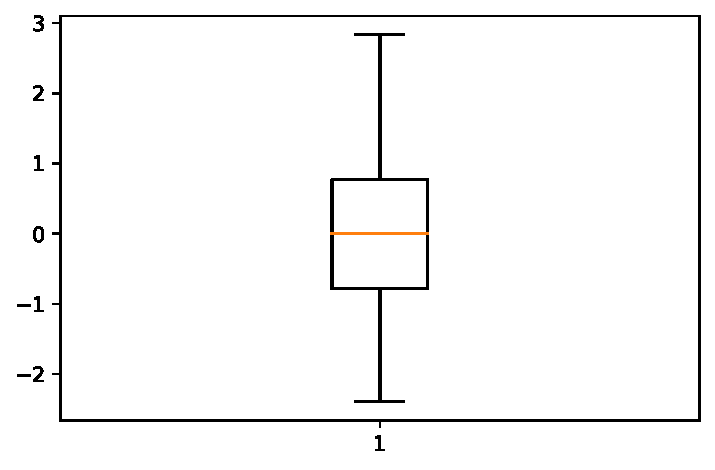
\includegraphics{index_files/figure-pdf/cell-2-output-1.pdf}

}

\end{figure}

En este ejemplo, cargamos nuestros datos y utilizamos la función
\texttt{boxplot()} de Matplotlib para crear el gráfico. Luego,
utilizamos \texttt{plt.show()} para mostrar el boxplot en una ventana
emergente.

\hypertarget{histogramas-y-distribuciones}{%
\subsection{Histogramas y
distribuciones}\label{histogramas-y-distribuciones}}

En el análisis de datos, es crucial comprender la distribución de
nuestros datos para obtener información valiosa. Una herramienta visual
poderosa para explorar la distribución es el histograma.

Un histograma es un gráfico de barras que muestra la frecuencia de
aparición de diferentes valores en un conjunto de datos. La variable que
estamos analizando se divide en intervalos y se representa en el eje x,
mientras que la frecuencia se muestra en el eje y. Cada barra representa
la cantidad de valores dentro de un intervalo específico.

Al observar un histograma, podemos identificar rápidamente la forma y la
simetría de la distribución de nuestros datos. Podemos detectar si los
datos siguen una distribución normal, están sesgados hacia la derecha o
hacia la izquierda, o si tienen múltiples picos. Esto nos proporciona
información valiosa sobre la naturaleza de nuestros datos y nos ayuda a
tomar decisiones informadas.

Para crear un histograma, podemos utilizar bibliotecas como Matplotlib y
Seaborn. Estas bibliotecas ofrecen funciones sencillas para generar
histogramas y personalizar su apariencia.

Aquí tienes un ejemplo básico de cómo crear un histograma utilizando
Matplotlib:

\begin{Shaded}
\begin{Highlighting}[]
\CommentTok{\# Cargar datos}
\NormalTok{data }\OperatorTok{=}\NormalTok{ np.random.randn(}\DecValTok{100}\NormalTok{)}

\CommentTok{\# Crear histograma}
\NormalTok{plt.hist(data, bins}\OperatorTok{=}\DecValTok{10}\NormalTok{)  }\CommentTok{\# bins representa el número de intervalos}

\CommentTok{\# Mostrar el histograma}
\NormalTok{plt.show()}
\end{Highlighting}
\end{Shaded}

\begin{figure}[H]

{\centering 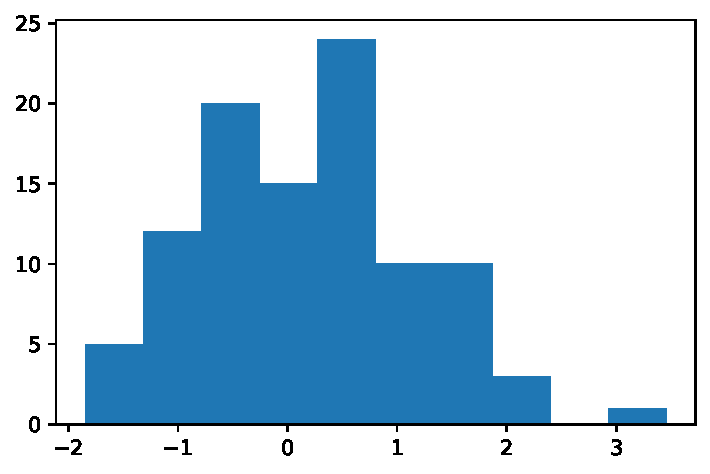
\includegraphics{index_files/figure-pdf/cell-3-output-1.pdf}

}

\end{figure}

En este ejemplo, cargamos nuestros datos y utilizamos la función
\texttt{hist()} de Matplotlib para crear el histograma. El parámetro
\texttt{bins} nos permite especificar el número de intervalos en los que
queremos dividir nuestros datos.

\hypertarget{gruxe1ficos-de-correlaciuxf3n}{%
\subsection{Gráficos de
correlación}\label{gruxe1ficos-de-correlaciuxf3n}}

Cuando trabajamos con conjuntos de datos, a menudo queremos explorar la
relación entre diferentes variables. Los gráficos de correlación nos
permiten visualizar esta relación y determinar si existe una conexión
significativa entre las variables.

Un gráfico de correlación muestra cómo se relacionan dos variables entre
sí. Nos ayuda a identificar patrones y tendencias, así como la fuerza y
dirección de la relación. El coeficiente de correlación nos proporciona
una medida numérica de la relación, donde valores cercanos a 1 indican
una correlación positiva, valores cercanos a -1 indican una correlación
negativa, y valores cercanos a 0 indican una correlación débil o
inexistente.

Una forma común de representar gráficamente la correlación es mediante
un diagrama de dispersión. En este tipo de gráfico, cada punto
representa una observación en el conjunto de datos, y su posición en el
plano cartesiano refleja los valores de las dos variables. Si los puntos
tienden a formar una línea ascendente o descendente, indica una
correlación positiva o negativa, respectivamente.

Para crear un gráfico de correlación, podemos utilizar bibliotecas como
Matplotlib y Seaborn. Estas bibliotecas nos ofrecen funciones sencillas
para generar diagramas de dispersión y calcular los coeficientes de
correlación.

Aquí tienes un ejemplo básico de cómo crear un gráfico de correlación
utilizando Seaborn:

\begin{Shaded}
\begin{Highlighting}[]
\CommentTok{\# pip install seaborn}
\CommentTok{\# pip install matplotlib}


\CommentTok{\# Cargar datos}
\NormalTok{data }\OperatorTok{=}\NormalTok{ pd.DataFrame(\{}\StringTok{\textquotesingle{}variable1\textquotesingle{}}\NormalTok{: [}\DecValTok{1}\NormalTok{, }\DecValTok{2}\NormalTok{, }\DecValTok{3}\NormalTok{, }\DecValTok{4}\NormalTok{, }\DecValTok{5}\NormalTok{],}
                     \StringTok{\textquotesingle{}variable2\textquotesingle{}}\NormalTok{: [}\DecValTok{2}\NormalTok{, }\DecValTok{4}\NormalTok{, }\DecValTok{6}\NormalTok{, }\DecValTok{8}\NormalTok{, }\DecValTok{10}\NormalTok{]\})}

\CommentTok{\# Crear gráfico de correlación}
\NormalTok{sns.scatterplot(x}\OperatorTok{=}\NormalTok{data[}\StringTok{\textquotesingle{}variable1\textquotesingle{}}\NormalTok{], y}\OperatorTok{=}\NormalTok{data[}\StringTok{\textquotesingle{}variable2\textquotesingle{}}\NormalTok{])}

\CommentTok{\# Mostrar el gráfico}
\NormalTok{plt.show()}
\end{Highlighting}
\end{Shaded}

\begin{figure}[H]

{\centering 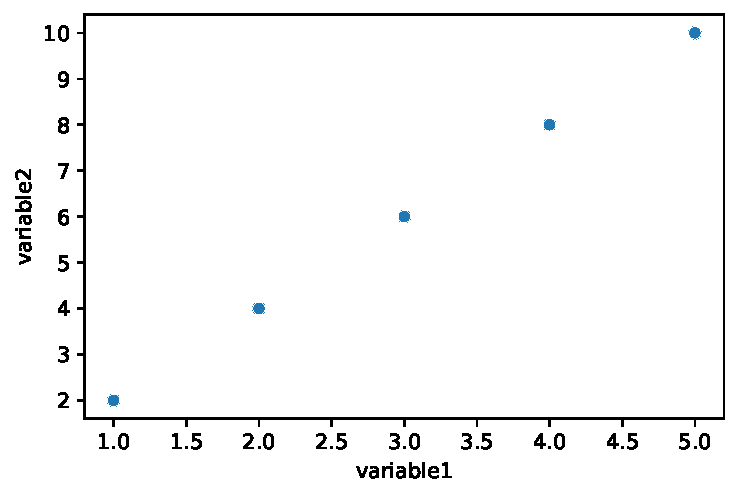
\includegraphics{index_files/figure-pdf/cell-4-output-1.pdf}

}

\end{figure}

En este ejemplo, cargamos nuestros datos y utilizamos la función
\texttt{scatterplot()} de Seaborn para crear el gráfico de correlación.
Simplemente especificamos las variables que queremos comparar en los
ejes x e y.

\hypertarget{publicaciones-similares}{%
\section{Publicaciones Similares}\label{publicaciones-similares}}

Si te interesó este artículo, te recomendamos que explores otros blogs y
recursos relacionados que pueden ampliar tus conocimientos. Aquí te dejo
algunas sugerencias:


\printbibliography


\end{document}
